\title{Rayleigh–Bénard convection - Project report} %07/nov/2014

\documentclass[12pt,oneside]{article}
\usepackage{amsmath,amssymb,amsthm}
\usepackage[english]{babel}
\usepackage[utf8]{inputenc}  
\usepackage[T1]{fontenc}
\usepackage{graphicx}
\usepackage{lscape}
\usepackage[hmargin=2.5cm,vmargin=2.5cm,bmargin=2.5cm]{geometry}
\usepackage{caption}
\usepackage{subcaption}
\usepackage{hyperref}
\usepackage{bbm}
\usepackage{cancel}

\usepackage{freefem}
\lstset{language=freefem++}

\newcommand{\hey}[1]{\LARGE \color{red}{#1}}

\newcommand{\ddt}[1]{\displaystyle\frac{\partial {#1}}{\partial t}} 	% Material derivative
\newcommand{\DDt}[1]{\displaystyle\frac{D {#1}}{D t}} 					% Time derivative
\newcommand{\divergence}[1]{\nabla\cdot{#1}} 							% Divergence
\newcommand{\gradient}[1]{\nabla{#1}} 									% Gradient
\newcommand{\laplacian}[1]{\nabla^2{#1}} 								% Laplacian

\newcommand\Rey{\mbox{\textit{Re}}}  									% Reynolds number
\newcommand\Pra{\mbox{\textit{Pr}}} 									% Prandtl number
\newcommand\Ray{\mbox{\textit{Ra}}}  									% Rayleigh number

\newcommand\intO{\displaystyle\int_\Omega}								% Integral over \Omega

\renewcommand{\thefigure}{\arabic{section}.\arabic{figure}}

\setcounter{secnumdepth}{2}

\begin{document}
\baselineskip=1.5em
\thispagestyle{empty}

\begin{center}
{\Huge \bf École polytechnique}\\


\vspace{5cm}

{\LARGE{\bf Rayleigh–Bénard convection \\ }}
Project report

\vspace{6cm}
ROVINA DE ALMEIDA, Gabriel\\
\end{center}

\vspace{5cm}

\begin{center}
\textbf{Palaiseau, France \\  Novembre 2014}
\end{center}


%%%%%%%%%%%%%%%%%%%%%%%%%%%%%%%%%%%%%%%%%%%%%%%%%%
\newpage
\thispagestyle{empty}

\setcounter{tocdepth}{3}
\tableofcontents

\listoffigures

\newpage
\setcounter{page}{1}
%%%%%%%%%%%%%%%%%%%%%%%%%%%%%%%%%%%%%%%%%%%%%%%%%%
\section{Introduction}

Convective flows result from the combination of a gravitation field and an adverse temperature gradient. They are widely present in nature in the most diverse scales: the atmosphere, the Earth's mantle, room heating or cooling, the sun and even spaghetti cooking. They role are of great importance in and their behaviour can vary from completely still to instationary or even chaotic.

This project aims the simulation and analysis of a simple setting in which this phenomenon can be observed: the Rayleigh-Bénard convection. It consists of a fluid confined between two horizontal plates subjected to an adverse temperature gradient. Under specific conditions, this configuration may present instability and originate the convection process.

The main actors in this phenomenon are the buoyant forces and the viscous and thermal diffusions. Heat from the bottom plate is transferred to the fluid nearby, inducing thermal expansion and therefore the local density to be decreased. As a consequence, buoyancy pushes the lighter fluid upwards. At the same time, the heavier fluid on the upper part tends to go down.

This effect tends to be attenuated by viscosity and therefore only takes place beyond a certain threshold value of the control parameters.
For the situation when these masses are moved, heat can be exchanged with their new neighbours and other cycles can happen.

We can then predict two main scenarios: the first one, when dissipation effects are predominant, consists of a steady temperature gradient from bottom to top, conducting heat in a continuous and uniform way. A good example is found in solids (Figure \ref{fig:solid}), for which viscosity is infinitely greater than any buoyant effect.

\begin{figure}[ht]
  \centering
  \begin{subfigure}[b]{0.4\textwidth}
    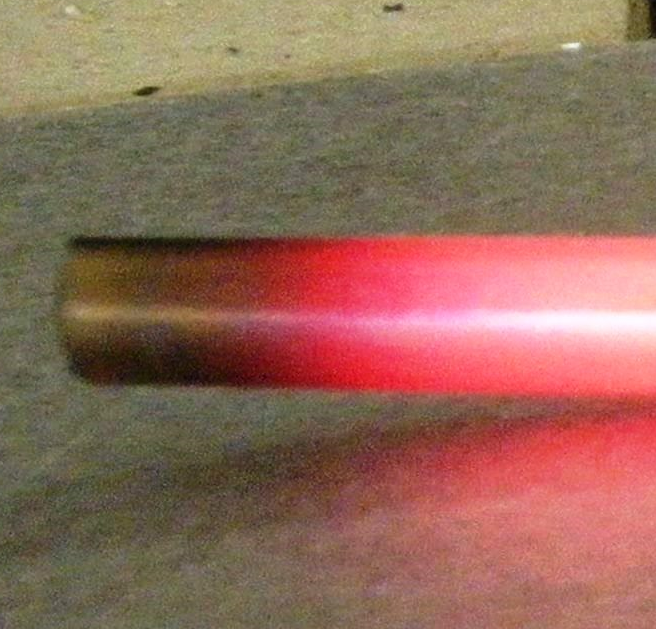
\includegraphics[width=\textwidth]{solid}
    \caption{Solid conduction}
    \label{fig:solid}
  \end{subfigure}
  \quad
  \begin{subfigure}[b]{0.4\textwidth}
    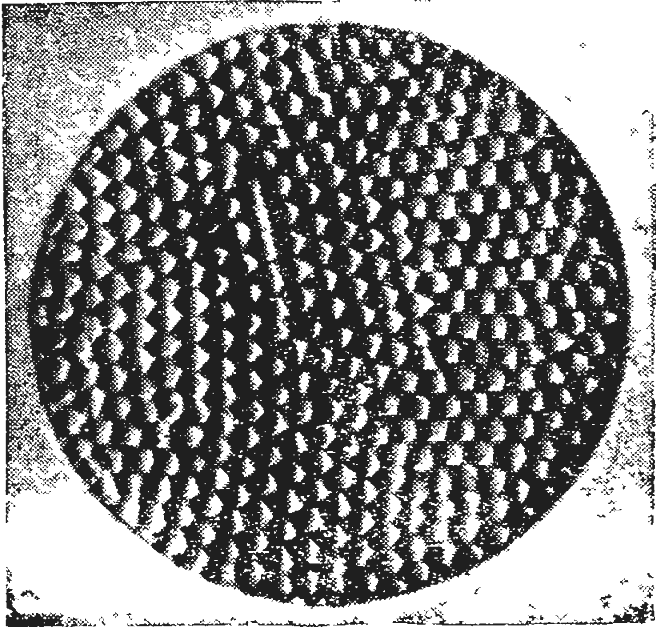
\includegraphics[trim=1cm 2cm 1cm 2cm, clip=true, width=\textwidth]{benard}
    \caption{Bénard cells (reproduction from \cite{benard})}
    \label{fig:benard}
  \end{subfigure}
  \caption{Two expected scenarios}\label{fig:scenarios}
\end{figure}

Another situation is expected to set up when buoyant forces are the ones in charge. In this second case, a constant version of the moving masses explained above is expected: fluid may constantly perform convective cycles and exchange heat near the plates.

The convections studied by Bénard in {\it Les tourbillons cellulaires dans une nappe liquide} fit indeed this last description. In his configurations, the motion happens in convective cells (Bénard cells), and flow alternates between the two plates in a relatively organised manner.

%%%%%%%%%%%%%%%%%%%%%%%%%%%%%%%%%%%%%%%%%%%%%%%%%%
\section{Modelling}
The scheme in Figure \ref{fig:scheme} represents the studied situation. Temperature on the bottom and on the top plates are fixed respectively as $\theta_a$ and $\theta_b$.

\begin{figure}[ht]
 \centering
 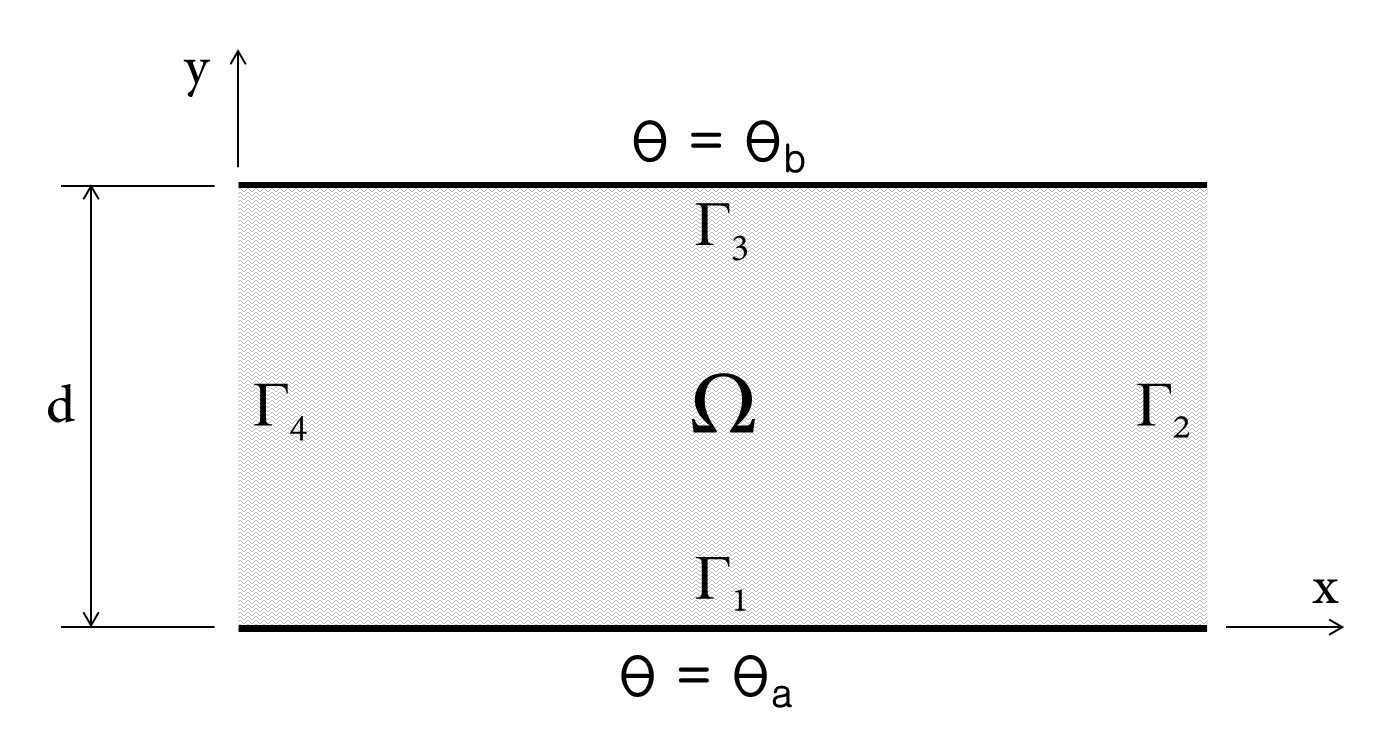
\includegraphics[width=0.75\textwidth]{scheme}
 \caption{Scheme}
 \label{fig:scheme}
\end{figure}

Both plates are considered as no-slip impermeable surfaces. The situation of infinite surfaces is reduced to a limited domain to possibilitate the simulation. This demands special attention while choosing boundary conditions for side walls.


\subsection{Equations}
We start from the full compressible Navier-Stokes equations for a Newtonian fluid assuming that changes in temperature are moderated, so that we can consider the coefficients as constants:

\begin{equation}\nonumber\left\{
\begin{array}{l}
\DDt{(\rho\bf{u})} = \mu \laplacian{\bf{u}} + (\lambda + \mu) \, \gradient{(\divergence{\bf{u}})} - \gradient{p} + {\bf{f}} \\[10pt]
\DDt{\rho} = - \rho \, \divergence{\bf{u}}
\end{array}\right.
\end{equation}

where $\DDt{\bf{a}} := \ddt{\bf{a}} + (\bf{u}\cdot \nabla)\bf{a}$ represents the material derivative of the field $\bf{a}$; $\rho$ stands for the density; $\bf{u}$, the velocity; $\mu$, the dynamic viscosity and $p$, the pressure.

The term $f$ takes into account the external force, given in this case by the gravitational contribution and thus defined as:
$$f = \rho \, \bf{g} = - \rho \, g \, \bf{e_y}$$

Following the Oberbeck-Boussinesq model (\cite{chandra}), we suppose that variations in density are very small and only due to thermal behaviour so that we can consider the fluid as incompressible and condense these effects on the buoyancy term. For $\rho_0$ the reference density --- {\it{i.e.}} measured at the reference temperature $\theta_0$ ---, the new equations read:

\begin{equation}\nonumber\label{eq:nsdim}\left\{
\begin{array}{l}
\rho_0 \,\displaystyle\frac{D\bf{u}}{Dt} = \mu \laplacian{\bf{u}} - \gradient{p} - \rho \, g \, \bf{e_y} \\[12pt]
\divergence{\bf{u}}=0
\end{array}\right.
\end{equation}


The next step is introduced by the Boussinesq approximation, a first order expansion of the density variation around its reference value as a function of the temperature:
\begin{equation}
\rho = \rho_0 \, [1 - \alpha (\theta - \theta_0)]
\end{equation}
where the linear term $\alpha$ is called the thermal expansion coefficient.

Finally, for $\kappa$ being the thermal diffusivity of the fluid (adopted constant), we write the evolution equation for the temperature as a passive scalar:
\begin{equation}\label{eq:tempdim}
\DDt{\theta} = \kappa \laplacian{\theta}
\end{equation}


\subsubsection{Dimensionless form}

In order to reduce the number of parameters in equations \ref{eq:nsdim}--\ref{eq:tempdim}, we can define reference values for the studied quantities. Let them be: $d$ for distances, $d^2/\kappa$ for time, $\rho_0 \kappa^2 / d^2$ for pressures and $\theta_a-\theta_b =: \Delta \theta$ for temperature. We then introduce two additional changes of variable:
$$ \Delta \theta \, \theta' = \theta - \theta_0 \qquad
\text{and}
\qquad \frac{\rho_0 \kappa^2}{d^2} \, p' = p - \rho_0 \, g \, y $$

By applying these changes and redefining the quantities as a dimensionless prime quantity multiplied by its reference value, the equations \ref{eq:nsdim}--\ref{eq:tempdim} can be expressed in a dimensioless form\footnote{For the sake of readability, the primes on the operators are omitted.}:
\begin{equation}\label{eq:dimless}\left\{
\begin{array}{l}
\displaystyle\frac{D\bf{u'}}{Dt'} = \Pra \, \laplacian{\bf{u'}} - \gradient{p'} + \Ray \, \Pra \, \theta' \, \bf{e_y} \\[12pt]
\divergence{\bf{u'}}=0 \\[5pt]
\displaystyle\frac{D\theta'}{Dt'} = \laplacian{\theta'}
\end{array}\right.
\end{equation}

Here the value of $\theta_a$ is assimilated to the reference temperature $\theta_0$ and the two dimensionless groups $\mu / \rho_0 \, \kappa$ and $g \, \rho_0 \, \alpha \, \Delta \theta \, d^3 / \kappa \, \mu$ are respectively baptised the Prandtl number ($\Pra$) and the Rayleigh number ($\Ray$).

\subsubsection{Prandtl and Rayleigh numbers}

In the definition of the Prandtl number, we observe a ratio between two stabilising effects: the dynamic and the thermal viscosities. This factors are responsible for spreading respectively momentum and internal energy and diminishing instabilising concentration of quantities in the fluid. Therefore, even if the Prandtl number presents a great influence on the general behaviour of the fluid, it is not the determinant factor in what concerns the manifestation of instabilities on the system.

The Rayleigh number, on the other hand, compares the buoyancy term to the viscous ones and establishes in this way a relation between destabilising and stabilising effects. As a consequence, low values of $\Ray$ are related to stability of the flow, whereas high values may arouse behaviours of unstable, turbulent and chaotic natures.


\subsection{Boundary conditions}

Once the equations describing the evolution of the system are determined, different situations can be simulated by imposing appropriate boundary conditions.

The model prescribes impermeable walls with no-slip property. This implies respectively that the normal and the tangential components of $\bf{u}$ vanish close to the surfaces and thus simply that $\bf{u} = \bf{0}$ on the plates.

From a large space of possibilities, some interesting situations are hand-picked to be tested. Firstly, we can start gently by bringing back the example of spaghetti cooking and modeling a covered pan heated from bellow. The walls of the pan being impermeable and no-slip surfaces, we have homogeneous Dirichlet condition for the velocity on all the boundaries. Another possible configuration can be simulated if we dare to open the pan, letting free the upper boundary $\Gamma_3$.

Thirdly, we can also let free the side boundaries $\Gamma_2$ and $\Gamma_4$ (it could be called the frying pan); and then just put back the cover, without bringing back the walls. Going further, we can let free our imagination instead of the side boundaries, bending space and time in other to create a periodic boundary condition, connecting $\Gamma_2$ to $\Gamma_4$.




%%%%%%%%%%%%%%%%%%%%%%%%%%%%%%%%%%%%%%%%%%%%%%%%%%
\section{Implementation}

\subsection{The method of characteristics}
One of the main issues for implementing the Navier-Stokes equations is handling the non-linearity of the advection term. Explicit approaches are usually of easier implementation and enjoy good performance in a general way; the price being concentrated on poor stability characteristics. Taking this parameter into consideration, we have opted for the method of characteristics. It also offers an explicit treatment of the non-linear term, but presents nevertheless better stability properties than other regular explicit schemes.

This method can be interpreted as a time discretisation for the material derivative of a quantity. It computes, for a point on the grid, the rate of change not in relation to the same point, but to the value found on the position where the particle in this point was in the last step, as illustrated in Figure \ref{fig:charac}.

\begin{figure}[ht]
 \centering
 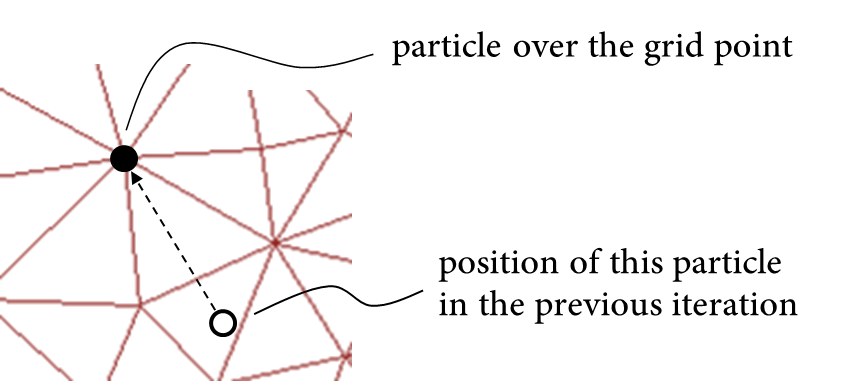
\includegraphics[width=0.65\textwidth]{charac}
 \caption{Method of characteristics}
 \footnotesize{Backwards integration in time is used to estimate the previous position of the particle.}
 \label{fig:charac}
\end{figure}

For this purpose, this method requires the integration of the velocity field backwards in time, finding in this way the previous position of the advected particle and then its velocity at that moment. Calling $X^n$ an operator that associates the position of a particle on the point $x$ to the position where it was on the previous time step --- \emph{estimated with $\bf{u}^n$} ---, we can then discretise the material derivative of a quantity $a$ in the following way:

\begin{equation}\label{eq:timedisc}
\frac{Da}{Dt'} = \frac{a^{n} - a^{n-1} \circ X^{n-1} }{\Delta t'} + \mathcal{O}(\Delta t')
\end{equation}
\emph{\small{Note that in order to have an explicit scheme, the operator $X$ is required to perform the backwards integration based on the known velocity field $\bf{u}^{n-1}$.}}
\\

Hence, this approach with the method of characteristics comprises not only a discretisation in time, but also a way around to treat the non-linearity, for the case of $a = \bf{u}$.

\subsection{Variational formulation}

Based on the governing set of equations \ref{eq:dimless} and on the time discretisation presented above (Equation \ref{eq:timedisc}) to the velocity and the temperature, we proceed to finding a variational formulation for the problem. We consider for this finality three compact support test functions: $\bf{v}$, for velocities; $q$, for pressure and $\tau$, for temperature.

We then take the scalar product between these functions and their respective equations and integrate over the domain:
\begin{equation}\nonumber\left\{
\begin{array}{l}
\intO \left( \displaystyle\frac{{\bf{u}^{n}} - {\bf{u}^{n-1}} \circ X^{n-1} }{\Delta t'} \, \cdot \, \bf{v} \right) d\Omega \; = \\[10pt]
\qquad \qquad = \intO \left( \Pra \, \laplacian{\bf{u}^n} \, \cdot \, {\bf{v}} - \gradient{p^n} \, \cdot \, \bf{v} + \Ray \, \Pra \, \theta^{n-1} \, \bf{e_y} \, \cdot \, \bf{v} \right) d\Omega \\[12pt]
\intO \divergence{\bf{u}^n} \, q \, d\Omega = 0 \\[14pt]
\intO \displaystyle\frac{\theta^{n} - \theta^{n-1} \circ X^{n-1} }{\Delta t'} \, \tau \, d\Omega   = \intO \laplacian{\theta^n} \, \tau \, d\Omega
\end{array}\right.
\end{equation}

\paragraph{Remark} For the cases in which we deal with Neumann conditions, the discussion of whether the term $^t\gradient{\bf{u}}$ should be considered arises. In fact, this term is not considered when we try to simulate an infinite domain between the plates, but is indeed taken into account for the case in which we let free the $\Gamma_3$ ("open pan" simulation).

\paragraph{Another remark} Following \cite{map559}, the finite elements were chosen as $P_2$ for the velocity and $P_1$ for pressure and temperature. This combination was troubled however in the cases implementing periodic domain, for which $P_2$ elements were chosen for all the quantities.


Here the first equation uses the known value $\theta^{n-1}$ of the temperature in order to maintain its explicitness. We can then work further on these equations by integrating by parts, remarking that the boundary terms vanish from the fact that we have compact support test functions. The set of equations finally writes:
\begin{equation}\left\{
\begin{array}{l}
\displaystyle\frac{1}{\Delta t'} \intO {\bf{u}}^n \, \cdot \, {\bf{v}} \, d\Omega - \displaystyle\frac{1}{\Delta t'} \intO {\bf{u}^{n-1}} \circ X^{n-1} \, \cdot \, {\bf{v}} \, d\Omega \; =\\[10pt] 
\qquad \qquad = - \Pra \intO \gradient{\bf{u}^n} : \gradient{\bf{v}} \, d\Omega + \intO p^n \, \divergence{\bf{v}} \, d\Omega + \Ray \, \Pra \intO \theta^{n-1} \, v_y \, d\Omega
\\[12pt]
\intO q \, \divergence{\bf{u}^n} \, d\Omega = 0 \\[14pt]
\intO \displaystyle\frac{\bf{\theta}^{n} - \bf{\theta}^{n-1} \circ X^{n-1} }{\Delta t'} \, d\Omega   = \intO \laplacian{\theta^n} \, \tau \, d\Omega
\end{array}\right.
\end{equation}


Once we have obtained the variational form of equations, we can finally proceed to the implementation in FreeFem++ and start to "play with fire".


\clearpage
%%%%%%%%%%%%%%%%%%%%%%%%%%%%%%%%%%%%%%%%%%%%%%%%%%
\section{Results}

\subsubsection{The delicate heating}
If we take low values of $\Ray$, solutions present a stable behaviour, since destabilising effects are amortised by viscous ones. The simulation results exhibited in Figure \ref{fig:delicate} exemplify this case and one can observe similarities with Figure \ref{fig:solid}.

\begin{figure}[ht]
 \centering
 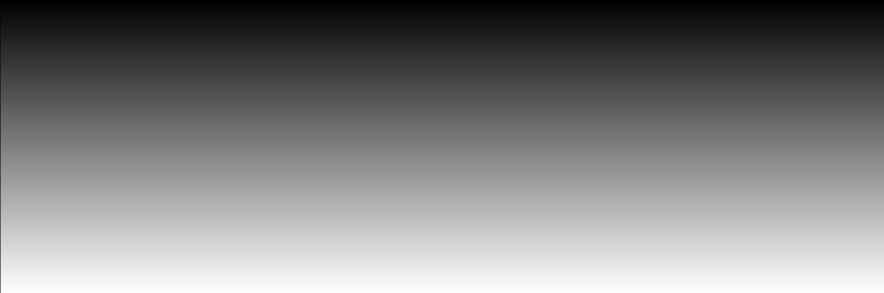
\includegraphics[width=0.95\textwidth]{09_0040t.png}
 \caption{Uniform temperature gradient for low Rayleigh number}
 \label{fig:delicate}
\end{figure}

As one may see, this profile corresponds to the first predicted scenario: a uniform and stable temperature gradient between the plates.

\paragraph{Pushing it beyond} However, if we then increase the $\Ray$ in a sudden way, the situation may change, as we can observe in Figure \ref{fig:push}.

\begin{figure}[ht]
 \centering
 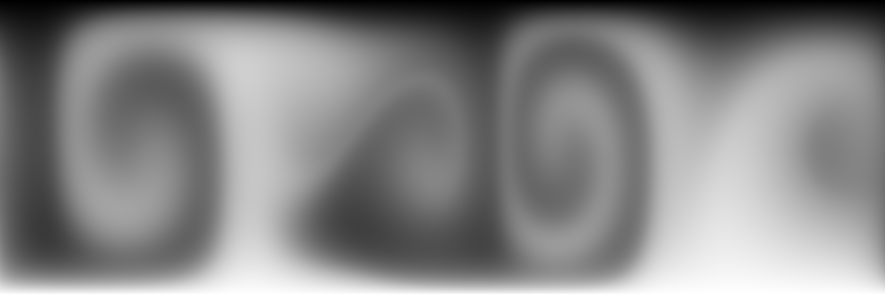
\includegraphics[width=0.95\textwidth]{15_0006t.png}
 \caption{Destabilising the uniform temperature gradient}
 \label{fig:push}
\end{figure}


\subsubsection{"Mushrooms"}
For a general unstable case, fluid may move in blobs, also in accordance to the predictions in the beginning of this document. These sub-domains of fluid move in mushroom-like regions (astonishingly well fitted to our spaghetti pretext).

\begin{figure}[ht]
 \centering
 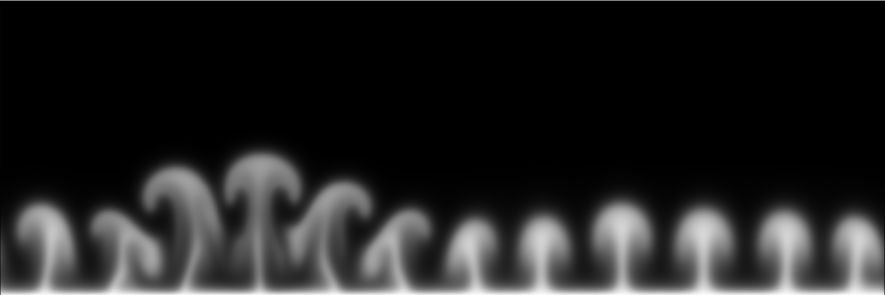
\includegraphics[width=0.95\textwidth]{14_0039t.png}
 \caption{The blooming of "mushrooms"}
 \label{fig:mush}
\end{figure}

This interesting shape can be explained by the presence of a couple of vortices that set up when the blob starts to climb. Figure \ref{fig:vort} shows "mushroom" in detail on both the temperature and the respective vorticity plots, unveiling the position of these vortices.

\begin{figure}[ht]
  \centering
  \begin{subfigure}[b]{0.48\textwidth}
    
\includegraphics[width=\textwidth]{vort1.png}
    \caption{Temperature}
  \end{subfigure}
  \begin{subfigure}[b]{0.48\textwidth}
    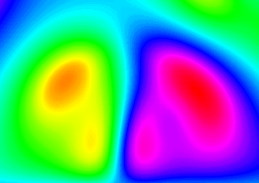
\includegraphics[width=\textwidth]{vort2.png}
    \caption{Vorticity}
  \end{subfigure}
  \caption{Vortices sculpting a mushroom}\label{fig:vort}
\end{figure}

The right vortex spins clockwise, while the left one spins anti-clockwise. We can also remark from the simulations the property that the predominant vortex tends to pull the mushroom towards its side. This way, we can predict that the mushroom in Figure \ref{fig:vort} is bending to the right.

\paragraph{Intertwining property}
In a general case, two mushrooms that get close to one another tend to get closer and closer and finally intertwine in a single one. As the situation in Figure \ref{fig:intert} illustrates, this union is not completely smooth and may cause some oscillations and small turbulence in the stalk.

\begin{figure}[ht]
 \centering
 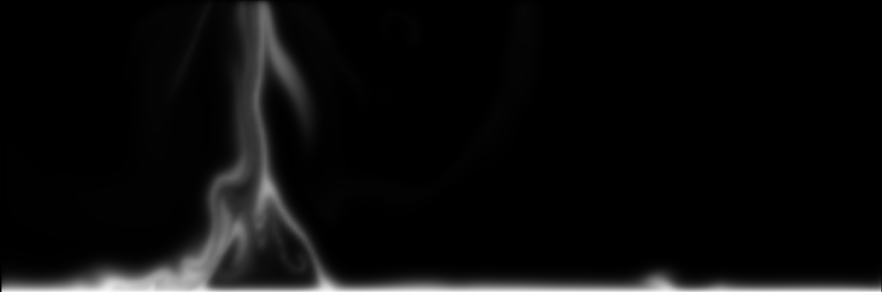
\includegraphics[width=0.95\textwidth]{06_0030t.png}
 \caption{Intertwining property}
 \label{fig:intert}
 \footnotesize{Simulation performed with free boundary conditions over $\Gamma_2 \cup \Gamma_3 \cup \Gamma_4$. and a no-slip impermeable surface in $\Gamma_1$}
\end{figure}

On the bottom of the picture, it is still possible to distinguish two filaments that come each one from a different mushroom. As the two blobs merge, their influence increase and it is relatively frequent to find the shown situation in which all the present mushrooms have been merged into a single one.

\subsubsection{The covered pan}
By setting null velocity along the four boundaries and the temperature bellow as unitary, we have the covered pan model. In this situation, turbulent flow is present and arising mushrooms are quickly mixed with the rest of the flow, as illustrates Figure \ref{fig:covpan}.

\begin{figure}[ht]
  \centering
  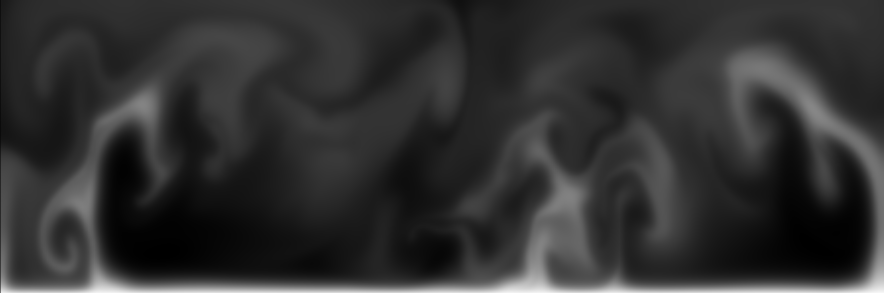
\includegraphics[width=.95\textwidth]{covpan2.png}
  \caption{Mixing in the covered pan}\label{fig:covpan}
\end{figure}

\subsubsection{The pre-heated situation}
For all the cases so far, initial temperature was taken as equal to $\theta_b$ everywhere. However, one of the most entertaining cases is the simulation of an initial average temperature over all the domain. This situation is shown in Figure \ref{fig:ave} for two moments in time.

\begin{figure}[ht]
  \centering
  \begin{subfigure}[b]{0.95\textwidth}
    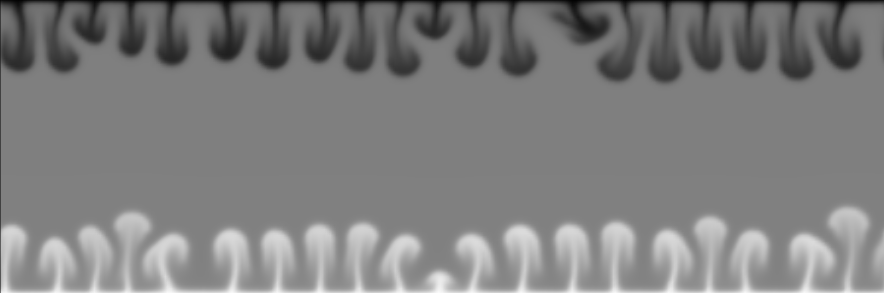
\includegraphics[width=\textwidth]{av1.png}
  \end{subfigure}
  \\[5pt]
  \begin{subfigure}[b]{0.95\textwidth}
    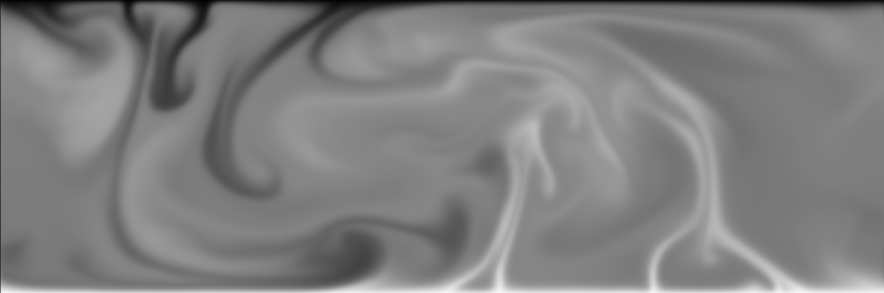
\includegraphics[width=\textwidth]{av2.png}
  \end{subfigure}
  \caption{Average temperature as initial condition}\label{fig:ave}
  \footnotesize{This simulation was performed with periodic boundary conditions}
\end{figure}

This time, we can notice the blooming of mushrooms from both plates and a clear example of the degree of unpredictability that the flow between these plates can achieve.

\subsubsection{The Bénard cell}
Finally, for the case of no friction on the walls, it was possible to observe the setup of Bénard cells after a certain time. The temperature and the velocity plots illustrated in Figure \ref{fig:bcell} show this circumstance that fits into our initial description of the situation when buoyant forces are in charge and a constant convective cycle takes place.

\begin{figure}[ht]
  \centering
  \begin{subfigure}[b]{0.95\textwidth}
    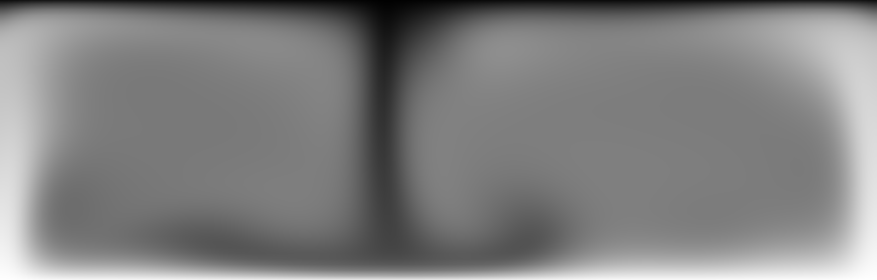
\includegraphics[width=\textwidth]{04_0201t.png}
    \caption{Temperature}
  \end{subfigure}
  \\
  \begin{subfigure}[b]{0.95\textwidth}
    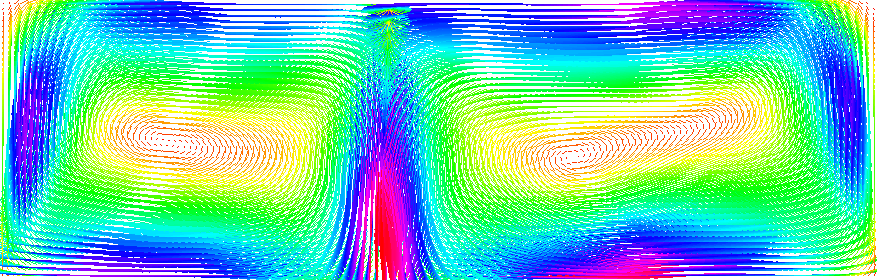
\includegraphics[width=\textwidth]{04_0201u.png}
    \caption{Velocity}
  \end{subfigure}
  \caption{Appearance of Bénard cells}\label{fig:bcell}
\end{figure}

We can observe in Figure \ref{fig:bcell} that two counter rotating vortices install a mechanism of heat exchange between upper and lower plates. Data from the rest of the simulation shows that this is a stable configuration, what makes this couple of vortices is fed by the temperature gradient and may last indefinitely once they set up.

%%%%%%%%%%%%%%%%%%%%%%%%%%%%%%%%%%%%%%%%%%%%%%%%%%
\section{Conclusion}

This project was above all surprising. It started off with a simple two-plate model that may have seemed uninteresting and inoffensive at first sight, but countless hidden properties of this system did not take long to pop out, such as organised structures, turbulent and chaotic behaviours, and beautiful mushroom-like blobs of fluid moving up and down.

On the other hand, the high complexity of the compressible Navier-Stokes equations with a force term depending on the "moving" variable $\theta$ could be handled by defining the appropriate set of hypothesis.

We could also shed light on the treatment of different combinations of boundary conditions and determine some working and some unrecommended approaches.

The satisfactory results and the simulation of a wide variety of situations not only indicate that the adopted hypothesis were reasonable for the tested situations, but also confirm the validity of the ensemble of settings and parameters chosen for the execution of the programme.

\enlargethispage{\baselineskip}
Altogether, the project was of great pertinence, in what concerns practical aspects of numerical fluid simulation; and of great interest, given the numerous amusing properties of the system of its solutions.

\clearpage
%%%%%%%%%%%%%%%%%%%%%%%%%%%%%%%%%%%%%%%%%%%%%%%%%%
\appendix
\section{FreeFem++ code}
\begin{lstlisting}
  // Parameters
  real Ra = 100*1708;	// Rayleigh number
  real Pr = 6.8;	// Prandtl number

  // Settings
  string prefix = "01";
  real dt = 1.e-3;	// time step
  real ds = 2.e-2;	// discretisation in space
  int steps = 250;	// number of iterations
  real L = 3.2;		// length of the box

  // Mesh
  mesh Mesh = square(L/ds,1/ds,[L*x,y]);
  plot(Mesh,ps=prefix+".png");

  // Vectorial spaces
  fespace Uspace(Mesh,P1b);	// for velocity
  fespace PTspace(Mesh,P1);	// for pressure and temperature

  // Variables
  Uspace	ux,tux,uxo=0.,
          uy,tuy,uyo=0.;
  PTspace	p,tp,
          t,tt,to=0.;
          
  // Auxiliar variables
  PTspace w;	// vorticity
  string msg, filename;
  bool draw;

  // Problems
  problem NavierStokes([ux,uy,p],[tux,tuy,tp]) =
      // eq1
       int2d(Mesh)( (ux*tux+uy*tuy)/dt )	// u / dt
      -int2d(Mesh)( (convect([uxo,uyo],-dt,uxo)*tux+convect([uxo,uyo],-dt,uyo)*tuy)/dt )	// - u0 o X / dt
      +int2d(Mesh)( Pr*(dx(ux)*dx(tux) +dy(ux)*dy(tux) +dx(uy)*dx(tuy) +dy(uy)*dy(tuy)) )
      //+int2d(Mesh)( Pr*(dx(ux)*dx(tux) +dx(uy)*dy(tux) +dy(ux)*dx(tuy) +dy(uy)*dy(tuy)) )	// - Pr \/2 u
      -int2d(Mesh)( p*(dx(tux)+dy(tuy)) )	// + \/p
      -int2d(Mesh)( Ra*Pr*to*tuy )	// - Ra * Pr * t * ey
      // eq2
      +int2d(Mesh)( tp*(dx(ux)+dy(uy)) )	// \/ . u
      // bc
      +on(1,3,ux=0.,uy=0.);
  
  problem Temperature([t],[tt]) =
      // eq3
       int2d(Mesh)( t*tt/dt ) // t / dt
      -int2d(Mesh)( convect([uxo,uyo],-dt,to)*tt/dt ) // -t0 o X / dt
      +int2d(Mesh)( dx(t)*dx(tt) +dy(t)*dy(tt) ) // - \/2 t
      // bc
      +on(1,t=1.);

  // Time march
  for (int i=1;i<=steps;i++) {

      msg = "Ra "+Ra+", Pr "+Pr+", step "+i;
      cout << msg << "/"+steps << endl;

      Temperature;
      to = t;
      
      NavierStokes;
      uxo = ux;
      uyo = uy;

      draw = true;
      if (draw) {
      	filename = prefix+"/";
        if (i<1e3) filename = filename+"0";
        if (i<1e2) filename = filename+"0";
        if (i<1e1) filename = filename+"0";
        filename = filename+i;
        
        // Velocity plot
        plot([ux,uy],cmm=msg,nbarrow=256,nbiso=256,ps="u/"+filename+".png",ArrowSize=-2.9);
        
		// Temperature plot
        plot(t,grey=1,cmm=msg,nbarrow=256,nbiso=256,fill=1,value=false,ps="t/"+filename+".png");
        
        // Vorticity computation and plot
      	w = dy(uxo)-dx(uyo);
        plot(w,cmm="Ra "+Ra+", Pr "+Pr+", step "+i,nbarrow=256,nbiso=256,fill=1,value=false,ps="w/"+filename+".png");
        
      }
  }
\end{lstlisting}

\clearpage
%%%%%%%%%%%%%%%%%%%%%%%%%%%%%%%%%%%%%%%%%%%%%%%%%%
\begin{thebibliography}{}

\bibitem{benard} Bénard H., {\it Les tourbillons cellulaires dans une nappe liquide}, Revue generale des sciences pures et appliquées, 1900.
\bibitem{map559} Alouges F., Maury B., {\it Variational Methods for Computation Fluid Dynamics} - Lecture notes.
\bibitem{chandra} Chandrasekhar S., {\it Hydrodynamic and hydromagnetic stability}. Clarendon Press, Oxford, 1961.
\bibitem{tallec} Le Tallec P., {\it Modélisation et calcul des milieux continus}, Éditions de l'École polytechnique, 2013.

\end{thebibliography}





\end{document}